\subsection{\texorpdfstring{Direct Image of a \(\tau\)-Extension}{Direct Image of a \textbackslash tau-Extension}}

Let G be a group, let F and \(F'\) be abelian groups, let \(\tau\) (resp. \(\tau'\) ) be a group homomorphism from G to the automorphism group of F (resp. \(F'\) ), and let \(v: F \to F'\) be a group homomorphism such that

\[
v (\tau (g) \cdot f) = \tau^ {\prime} (g) \cdot v (f)\tag{3}
\]

for every \(g \in G\) and \(f \in F\) . Let \(\mathcal{E} = (\Gamma, \iota, \pi)\) be a \(\tau\) -extension of G by F. Let \(\widetilde{\Gamma}\) be the external semidirect product \(F' \times_{\tau' \circ \pi} \Gamma\) . We denote by \(\widetilde{\iota}: F' \to \widetilde{\Gamma}\) the homomorphism \(f \mapsto (f, e)\) and by \(\widetilde{p}: \widetilde{\Gamma} \to \Gamma\) the first projection. Let \(j: F \to \widetilde{\Gamma}\) be the mapping defined by \(f \mapsto (v(f), \iota(f)^{-1})\) . Since the image of \(\iota\) is contained in the kernel of \(\tau' \circ \pi\) , the mapping j is a group homomorphism; it is injective because \(\iota\) is injective. We have the relations

\[
\begin{array}{r l} (f ^ {\prime}, \gamma) j (f) (f ^ {\prime}, \gamma) ^ {- 1} & = (f ^ {\prime}, \gamma) (v (f), \iota (f) ^ {- 1}) (f ^ {\prime}, \gamma) ^ {- 1} \\ & = (\tau^ {\prime} (\pi (\gamma)) \cdot v (f), \iota (\tau (\pi (\gamma)) \cdot f) ^ {- 1}) \\ & = j (\tau (\pi (\gamma)) \cdot f) \end{array}\tag{4}
\]

for \(f \in F\) , \(\gamma \in \Gamma\) , and \(f' \in F'\) . Consequently, the image of j is a normal subgroup of \(\widetilde{\Gamma}\) . We denote by \(\Gamma'\) the quotient of \(\widetilde{\Gamma}\) by the image of j. We denote by \(\iota'\) the composition of the canonical surjection from \(\widetilde{\Gamma}\) to \(\Gamma'\) and \(\widetilde{\iota}\) . The kernel of the homomorphism \(\pi \circ \widetilde{p}\) is the product \(\mathrm{F}' \times \iota(\mathrm{F})\) , which contains the image of j. We define \(\pi' : \Gamma' \to G\) as the group homomorphism deduced from \(\pi \circ \widetilde{p}\) by passing to the quotient. Since \(\iota\) is injective, the intersection of \(j(\mathrm{F})\) and \(\widetilde{\iota}(\mathrm{F}')\) is reduced to the identity element of \(\widetilde{\Gamma}\) ; it follows that \(\iota'\) is injective. The mapping from \(F' \times F\) to \(F' \times \iota(\mathrm{F}) = \operatorname{Ker}(\pi \circ \widetilde{p})\) given by

\[
(f ^ {\prime}, f) \longmapsto (f ^ {\prime} v (f), \iota (f) ^ {- 1})
\]

is a group isomorphism. The image of \(\iota'\) therefore coincides with the kernel of \(\pi'\) . Since \(\pi\) and \(\widetilde{p}\) are surjective, so is \(\pi'\) . This proves that \(\mathcal{E}' = (\Gamma', \iota, \pi')\) is a \(\tau'\) -extension of \(G\) by \(F'\) ; we call it the direct image of \(\mathcal{E}\) by \(v\) and denote it by \(v_{*}(\mathcal{E})\) . The composition of the canonical surjection from \(\widetilde{\Gamma}\) to \(\Gamma'\) and the group homomorphism from \(\Gamma\) to \(\widetilde{\Gamma}\) given by \(\gamma \mapsto (1, \gamma)\) is a group homomorphism \(\varphi : \Gamma \to \Gamma'\) that we call canonical.

PROPOSITION 2. --- In the notation above, the following diagram commutes:

\begin{enumerate}
\def\labelenumi{(\arabic{enumi})}
\setcounter{enumi}{4}
\tightlist
\item
\end{enumerate}

\pandocbounded{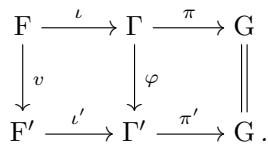
\includegraphics[keepaspectratio]{images/part002_f3abcdb3.jpg}}

Let \(\mathcal{E}_1' = (\Gamma_1', \iota_1', \pi_1')\) be a \(\tau'\) -extension of G by F', and let \(\varphi_1: \Gamma \to \Gamma_1'\) be a group homomorphism such that the following diagram commutes:

\pandocbounded{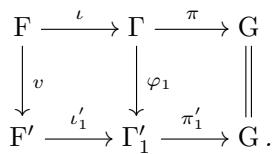
\includegraphics[keepaspectratio]{images/part002_c84edb93.jpg}}

Then there exists a unique morphism \(\psi\) of \(\tau'\) -extensions from \(v_{*}(\mathcal{E})\) to \(\mathcal{E}_1'\) such that we have \(\varphi_1 = \psi \circ \varphi\) .

The commutativity of the first diagram follows by construction. The existence and uniqueness of \(\psi\) follow from Lemma 3 below.

Lemma 3. --- Let \(G_{1}^{\prime}\) be a group, and let \(w: G \to G_{1}^{\prime}\) and \(\tau_{1}: G_{1}^{\prime} \to \operatorname{Aut}(F^{\prime})\) be group homomorphisms such that \(\tau^{\prime} = \tau_{1} \circ w\) . Let \(\mathcal{E}_{1}^{\prime} = (\Gamma_{1}^{\prime}, \iota_{1}^{\prime}, \pi_{1}^{\prime})\) be a \(\tau_{1}\) -extension of \(G_{1}^{\prime}\) by \(F^{\prime}\) , and let \(\varphi_{1}: \Gamma \to \Gamma_{1}^{\prime}\) be a group homomorphism such that the following diagram commutes:

\[
\begin{array}{c} \mathrm{F} \xrightarrow {\iota} \Gamma \xrightarrow {\pi} \mathrm{G} \\ \Biggl \downarrow_ {v} \qquad \qquad \Biggl \downarrow_ {\varphi_ {1}} \qquad \Biggl \downarrow_ {w} \\ \mathrm{F} ^ {\prime} \xrightarrow {\iota_ {1} ^ {\prime}} \Gamma_ {1} ^ {\prime} \xrightarrow {\pi_ {1} ^ {\prime}} \mathrm{G} _ {1} ^ {\prime}. \end{array}
\]

Then there exists a unique group homomorphism \(\psi : \Gamma' \to \Gamma'_1\) such that the diagram

\[
\begin{array}{c} \mathrm{F} ^ {\prime} \xrightarrow {\iota^ {\prime}} \Gamma^ {\prime} \xrightarrow {\pi^ {\prime}} \mathrm{G} \\ \Big \| \qquad \qquad \qquad \Big \downarrow_ {\psi} \qquad \Big \downarrow_ {w} \\ \mathrm{F} ^ {\prime} \xrightarrow {\iota_ {1} ^ {\prime}} \Gamma_ {1} ^ {\prime} \xrightarrow {\pi_ {1} ^ {\prime}} \mathrm{G} _ {1} ^ {\prime} \end{array}
\]

commutes and \(\varphi_{1} = \psi \circ \varphi\) .

For any \((f,\gamma)\in\mathrm{F}^{\prime}\times\Gamma\) , denote the class of \((f,\gamma)\) in \(\Gamma^{\prime}\) by \(\overline{(f,\gamma)}\) . If the group homomorphism \(\psi:\Gamma^{\prime}\to\Gamma_{1}^{\prime}\) has the desired properties, then it satisfies the relations

\[
\psi \big (\overline {{(f ^ {\prime} , \gamma)}} \big) = \psi (\iota^ {\prime} (f ^ {\prime}) \varphi (\gamma)) = \iota_ {1} ^ {\prime} (f ^ {\prime}) \varphi_ {1} (\gamma)
\]

for every \(f' \in \mathrm{F}'\) and \(\gamma \in \Gamma\) . Conversely, the mapping \(\tilde{\psi}\) from \(\mathrm{F}' \times_{\tau' \circ \pi} \Gamma\) to \(\Gamma_1'\) given by \((f, \gamma) \mapsto \iota_1'(f) \varphi_1(\gamma)\) is a group homomorphism. Indeed, we have the relations

\[
\begin{array}{r} \iota_ {1} ^ {\prime} (f) \varphi_ {1} (\gamma) \iota_ {1} ^ {\prime} (f ^ {\prime}) \varphi_ {1} (\gamma^ {\prime}) = \iota_ {1} ^ {\prime} (f \tau_ {1} (\pi_ {1} ^ {\prime} (\varphi_ {1} (\gamma))) \cdot f ^ {\prime}) \varphi_ {1} (\gamma \gamma^ {\prime}) \\ = \iota_ {1} ^ {\prime} (f \tau^ {\prime} (\pi (\gamma)) \cdot f ^ {\prime}) \varphi_ {1} (\gamma \gamma^ {\prime}) \end{array}
\]

for \(f, f' \in \mathrm{F}'\) and \(\gamma, \gamma' \in \Gamma\) . The kernel of \(\widetilde{\psi}\) contains the image of \(j\) because \(\iota_1'(v(f)) = \varphi_1(\iota(f))\) for \(f \in \mathrm{F}\) , and the morphism \(\psi\) deduced from \(\widetilde{\psi}\) by passing to the quotient has the desired properties.

Remark. --- Denote by \(\Sigma\) the species of structures of \(\tau'\) -extensions, and define \(\alpha\) -mappings to be mappings from \(\Gamma\) to a group \(\Gamma'\) underlying a \(\tau'\) -extension that are group homomorphisms and that make the following diagram commute:

\[
\begin{array}{c} \mathrm{F} \xrightarrow {\iota} \Gamma \xrightarrow {\pi} \mathrm{G} \\ \Big \downarrow v \qquad \qquad \Big \downarrow \varphi \\ \mathrm{F} ^ {\prime} \xrightarrow {\iota^ {\prime}} \Gamma^ {\prime} \xrightarrow {\pi^ {\prime}} \mathrm{G}. \end{array}\tag{6}
\]

Proposition 2 expresses that \(v_{*}(\mathcal{E})\) is a solution of the corresponding universal mapping problem (Set Theory, IV, §3, No.~1, p.~284).

COROLLARY 1. --- Let \(E_{1}\) and \(E_{2}\) be \(\tau\) -extensions of G by F, and let \(\psi\) be a morphism of \(\tau\) -extensions from \(E_{1}\) to \(E_{2}\) . Denote by \(\varphi_{1}\) (resp. \(\varphi_{2}\) ) the canonical homomorphism for \(v_{*}(\mathcal{E}_{1})\) (resp. \(v_{*}(\mathcal{E}_{2})\) ). Then there exists a unique morphism of \(\tau'\) -extensions from \(v_{*}(\mathcal{E}_{1})\) to \(v_{*}(\mathcal{E}_{2})\) , denoted by \(v_{*}(\psi)\) , such that \(\varphi_{2} \circ \psi = v_{*}(\psi) \circ \varphi_{1}\) .

It suffices to apply Proposition 2 to \(\varphi_{2} \circ \psi\) .

The class of the \(\tau^{\prime}\) -extension \(v_{*}(\mathcal{E})\) therefore depends only on the class of E. We also denote by \(v_{*}:\operatorname{Ex}_{\tau}(\mathrm{G},\mathrm{F})\to\operatorname{Ex}_{\tau^{\prime}}(\mathrm{G},\mathrm{F}^{\prime})\) the mapping that sends the class of a \(\tau\) -extension E to the class of the \(\tau^{\prime}\) -extension \(v_{*}(\mathcal{E})\) .

COROLLARY 2. --- We keep the notation of the proposition. Let F'' be an abelian group, and let \(\tau'' : G \to \text{Aut}(F'')\) and \(v': F' \to F''\) be group homomorphisms such that

\[
\tau^ {\prime \prime} (g) \cdot v ^ {\prime} (f) = v ^ {\prime} (\tau^ {\prime} (g) \cdot f)
\]

for \(g \in G\) and \(f \in F'\) . Let E be a \(\tau\) -extension of G by F, and denote by \(\varphi\) (resp. \(\varphi'\) , \(\varphi''\) ) the canonical homomorphism associated with \(v_{*}(\mathcal{E})\) (resp. \(v_{*}'(v_{*}(\mathcal{E}))\) , \((v' \circ v)_{*}(\mathcal{E})\) ). Then there exists a unique morphism \(\psi\) from the \(\tau''\) -extension \(v_{*}'(v_{*}(\mathcal{E}))\) of G by \(F''\) to the \(\tau''\) -extension \((v' \circ v)_{*}(\mathcal{E})\) such that \(\varphi'' = \psi \circ \varphi' \circ \varphi\) .

Examples. --- 1) Let \(j: \{1\} \to \mathrm{F}\) be the canonical injection. The semitrivial extension \(\mathcal{I}_{\tau}\) is isomorphic to \(j_{*}((\mathrm{G}, i, \mathrm{Id}_{\mathrm{G}}))\) , where \(i: \{e\} \to \mathrm{G}\) is the canonical injection. Let \(c: \mathrm{F} \to \mathrm{F}\) be the constant homomorphism \(f \mapsto 1\) , and let \(\mathcal{E}\) be a \(\tau\) -extension. The \(\tau\) -extension \(c_{*}(\mathcal{E})\) is also isomorphic to \(\mathcal{I}_{\tau}\) .

\begin{enumerate}
\def\labelenumi{\arabic{enumi})}
\setcounter{enumi}{1}
\tightlist
\item
  Let E be a subgroup of F stable under the action of G. Denote by \(F'\) the quotient of F by E, by \(v : F \to F'\) the canonical homomorphism, and by \(\tau' : G \to \text{Aut}(F')\) the action of G on \(F'\) characterized by
\end{enumerate}

\[
\tau^ {\prime} (g) \cdot v (f) = v (\tau (g) \cdot f)
\]

for \(g \in G\) and \(f \in F\) . Let \(\mathcal{E} = (\Gamma, \iota, \pi)\) be a \(\tau\) -extension of G by F. Then \(\iota(\mathrm{E})\) is a normal subgroup of \(\Gamma\) , and the \(\tau'\) -extension \(v_{*}(\mathcal{E})\) of G by \(F'\) is isomorphic to the extension \((\Gamma/\iota(\mathrm{E}), \bar{\iota}, \overline{\pi})\) , where \(\bar{\iota}\) and \(\overline{\pi}\) are the group homomorphisms deduced from \(\iota\) and \(\pi\) by passing to the quotients. By this isomorphism, the canonical homomorphism \(\varphi\) associated with \(v_{*}(\mathcal{E})\) corresponds to the canonical homomorphism from \(\Gamma\) to \(\Gamma/\iota(\mathrm{E})\) .

PROPOSITION 3. --- Let G and G' be groups, and let F and F' be abelian groups. Let \(\tau: \mathrm{G} \to \mathrm{Aut}(\mathrm{F})\) , \(\tau': \mathrm{G} \to \mathrm{Aut}(\mathrm{F}')\) , \(u: \mathrm{G}' \to \mathrm{G}\) , and \(v: \mathrm{F} \to \mathrm{F}'\) be group homomorphisms such that

\[
\tau^ {\prime} (g) \cdot v (f) = v (\tau (g) \cdot f)
\]

for \(g \in G\) and \(f \in F\) . We write \(\tau'' = \tau' \circ u\) . Let E be a \(\tau\) -extension of G by F. We denote by \(\varphi_u\) (resp. \(\varphi_v\) , \(\varphi'_u\) , \(\varphi'_v\) ) the canonical homomorphism corresponding to the \(\tau \circ u\) -extension \(u^*(\mathcal{E})\) (resp. to the \(\tau'\) -extension \(v_*(\mathcal{E})\) , to the \(\tau''\) -extensions \(u^*(v_*(\mathcal{E}))\) and \(v_*(u^*(\mathcal{E})))\) ). Then there exists a unique morphism \(\psi\) of \(\tau''\) -extensions from \(v_*(u^*(\mathcal{E}))\) to \(u^*(v_*(\mathcal{E}))\) such that \(\varphi_v \circ \varphi_u = \varphi'_u \circ \psi \circ \varphi'_v\) .

We denote the \(\tau \circ u\) -extension \(u^{*}(\mathcal{E})\) (resp. the \(\tau''\) -extension \(u^{*}(v_{*}(\mathcal{E}))\) ) by \((\Gamma_u, \iota_u, \pi_u)\) (resp. \((\Gamma_u', \iota_u', \pi_u')\) ). Applying Lemma 2 of VIII, p.~287 to \(\varphi_v \circ \varphi_u\) , we find that there exists a group homomorphism \(\psi_{1}:\Gamma_{u}\to\Gamma_{u}^{\prime}\) such that the diagram

\pandocbounded{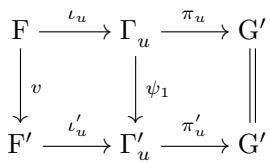
\includegraphics[keepaspectratio]{images/part002_ccea47d6.jpg}}

commutes and \(\varphi_{u}^{\prime}\circ\psi_{1}=\varphi_{v}\circ\varphi_{u}\) . The existence of \(\psi\) follows from Proposition 2 applied to \(\psi_{1}\) . Conversely, if \(\psi^{\prime}\) also has the desired properties, then we have \(\psi^{\prime}\circ\varphi_{v}^{\prime}=\psi_{1}\) by Lemma 2, so \(\psi^{\prime}=\psi\) (Proposition 2).

